The results shown in this section are obtained in standard fRG using an interaction cutoff: $G_0^\Lambda = \Lambda G_0$. The calculations are performed on the Matsubara frequency axis for temperature $T=0,08 t$, where $t$ is the nearest neighbors hopping.  

Besides the vertex, we have computed the susceptibilities, whose divergences follow the vertex ones. 

\subparagraph{Technicalities}
\begin{itemize} 

\item The vertex was decomposed in channels (magnetic, density, and superconducting) as in the literature \cite{Husemann2009, Husemann2012}, but we also kept fully the frequency dependence in a box. 

\item The momentum dependence of the vertex is treated by means of a form factor decomposition, while keeping 29 patches in the respective bosonic momentum transfer . The critical scale is fixed by the condition that the absolute value of one of the channels exceeds a value of 300$D$, $D=4t$. 


\item If not specified otherwise we did not include the self-energy feedback. 

\item The self energy flow results still numerically unstable.  
 
If not otherwise specified we measure energies in units of $D=4t$, i.e., $t'=-0.1$ corresponds to $t'=-0.4t$.
\end{itemize} 
 
\subparagraph{Results} 

In Fig \ref{phasediag_van_hove} and \ref{phasediag_van_hove_plus} we show  the critical scale as a function of $t'$, for, respectively, van Hove filling, and van Hove filling plus 7\%.    

The finite temperature acts as a cutoff for divergences in the bare bubble. 

In Fig. \ref{phasediag_van_hoveSTATIC} we show the same but for a static vertex, and for a temperature $T= 0.02t$. 
\begin{figure}
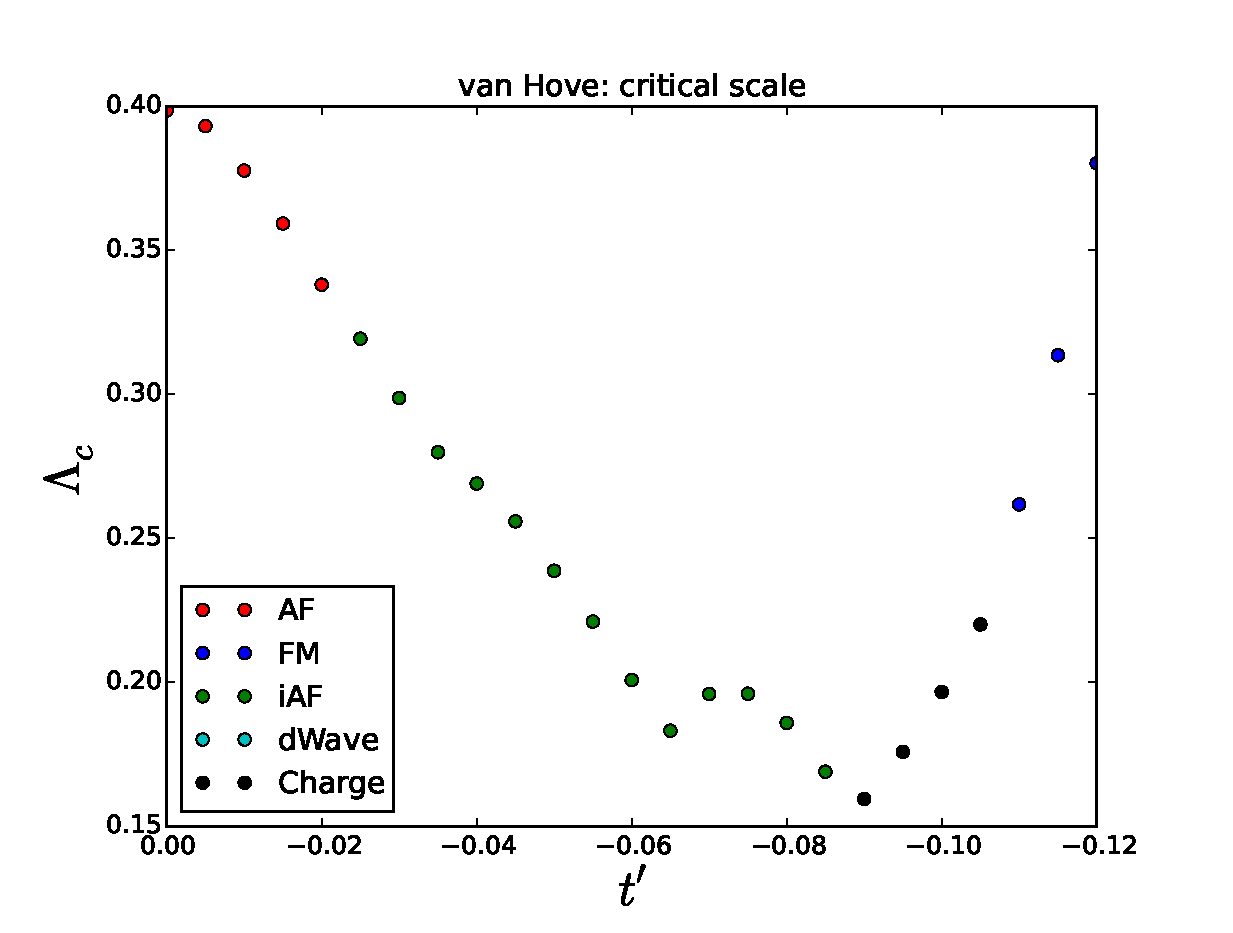
\includegraphics[scale=0.7]{vanHove_scan_critical_lambda_phi.eps}
\caption{Critical scale in full frequency fRG (interaction cutoff) as a function of the nearest neighbors hopping and for van Hove filling. The color of the symbol indicates the kind of instability that is realized.  } \label{phasediag_van_hove}

\end{figure}


\begin{figure}
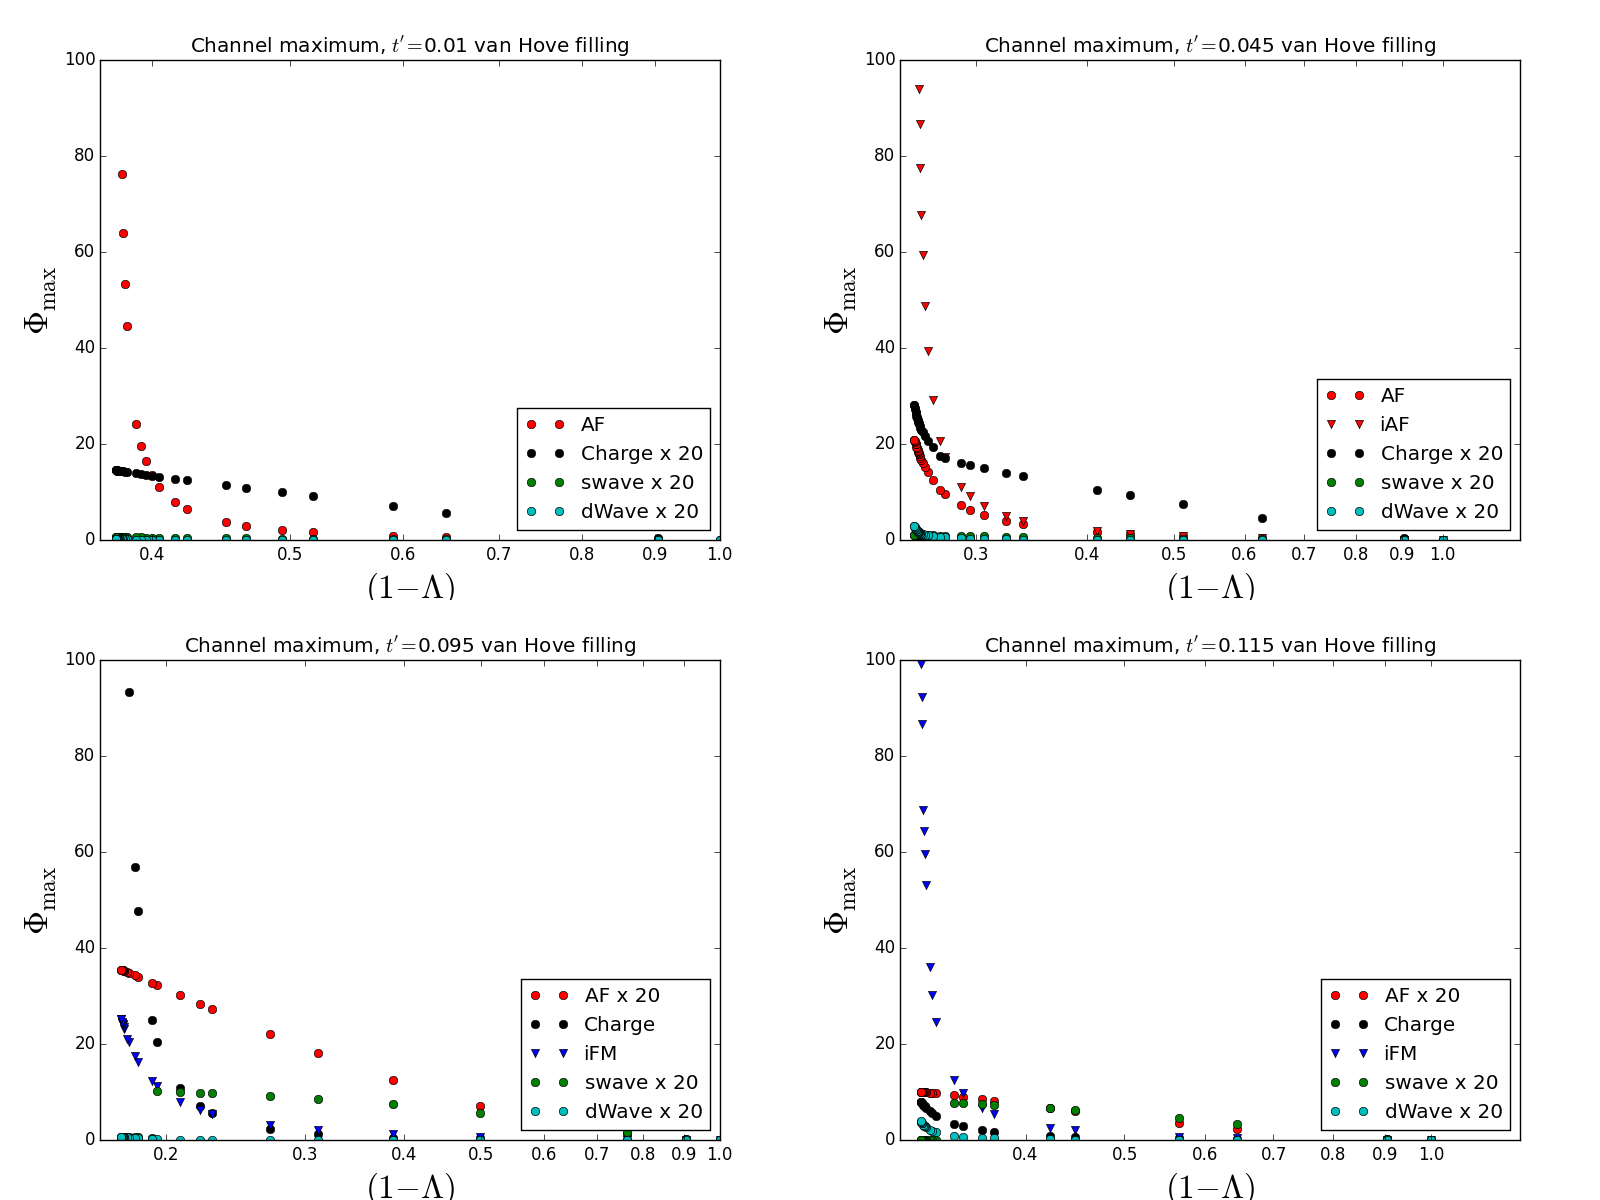
\includegraphics[scale=0.32,angle = 90]{images/vanhovelam.png}
\caption{Flow of the maximum of the absolute value of each channel for different values of $t'$ and at van Hove filling.
} 
\label{lamvan} 
\end{figure}


\begin{figure}
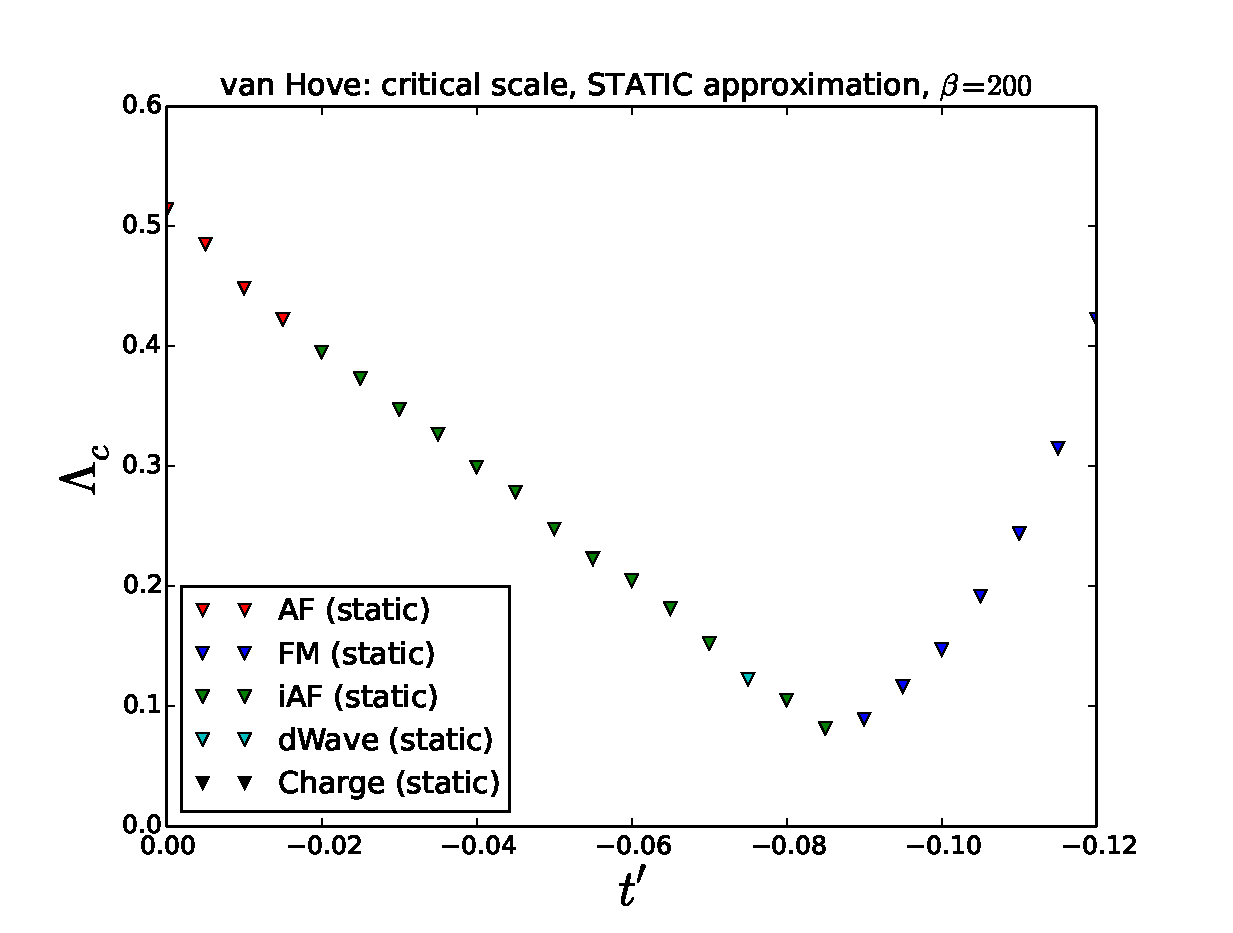
\includegraphics[scale=0.7]{images/vanHove_scan_critical_lambda_phiSTATIC.eps}
\caption{Critical scale in static fRG (interaction cutoff) as a function of the nearest neighbors hopping and for van Hove filling. The color of the symbol indicates the kind of instability that is realized.} 
\label{phasediag_van_hoveSTATIC} 
\end{figure}


\begin{figure}
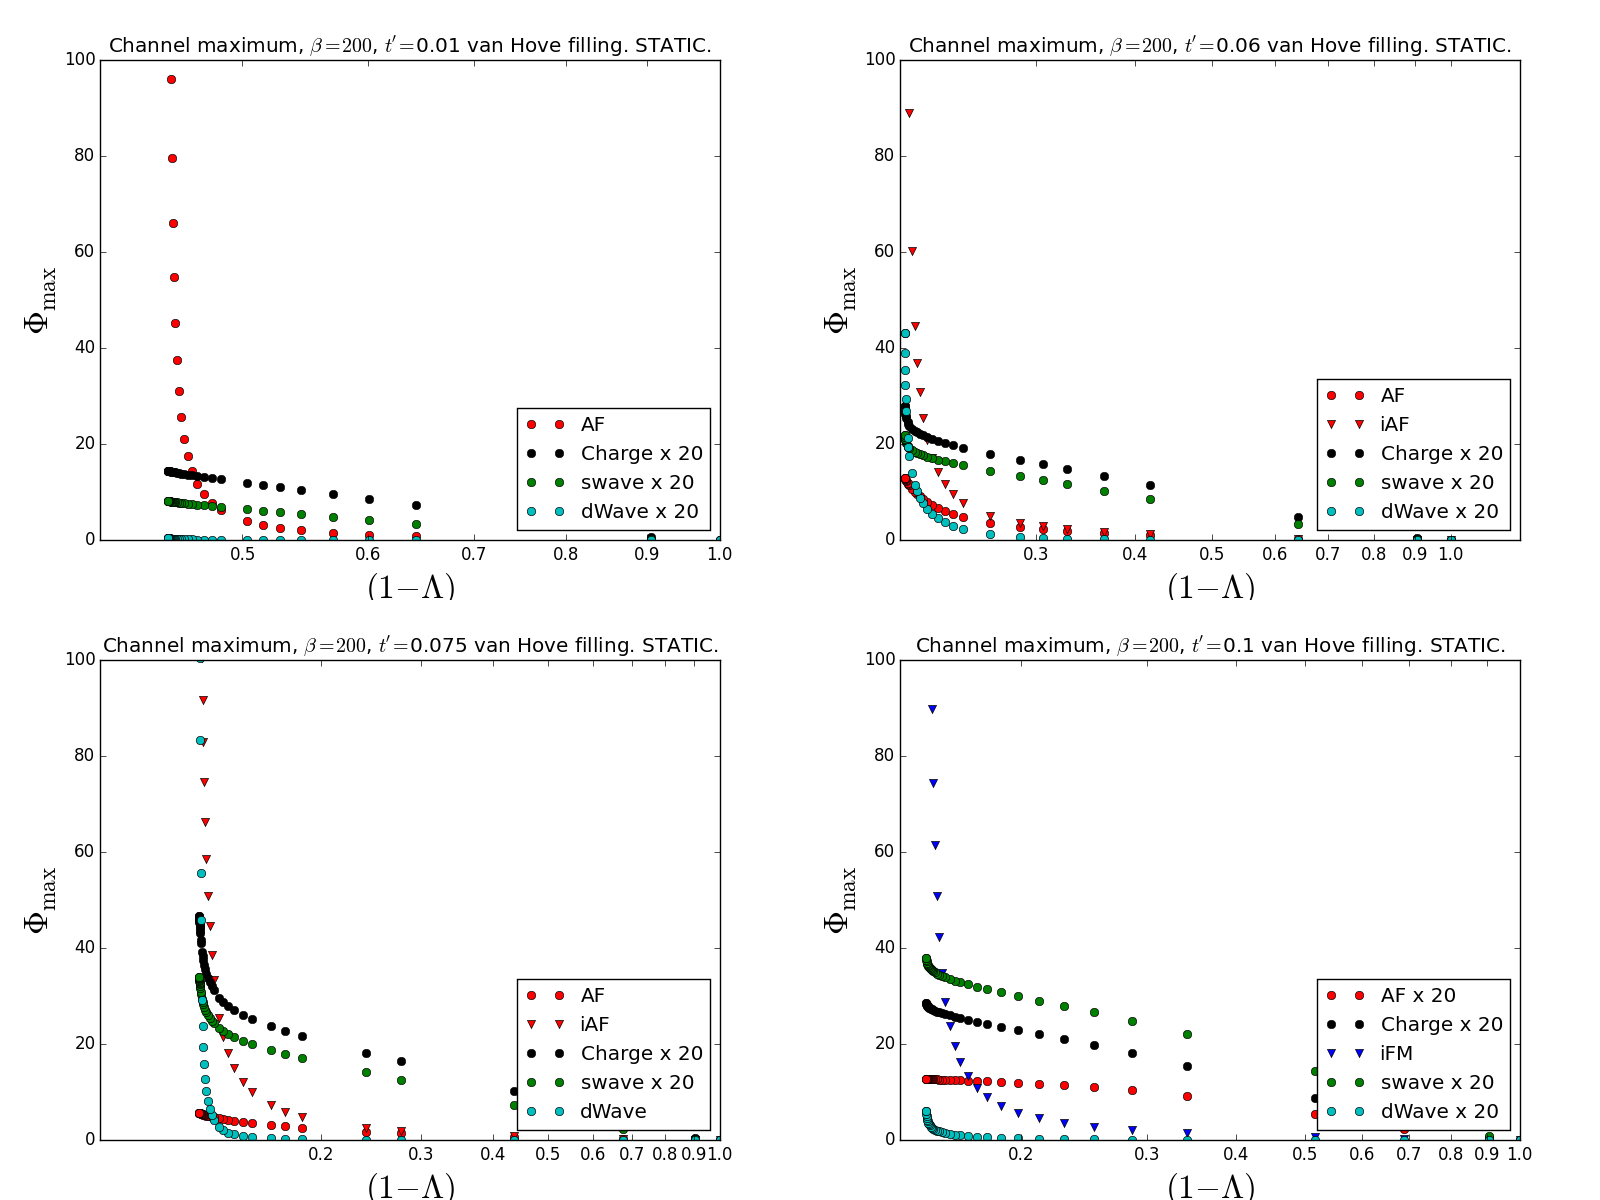
\includegraphics[scale=0.32,angle = 90]{images/static.png}
\caption{Flow of the maximum of the absolute value of each channel for different values of $t'$ and at van Hove filling, in the static approximation for the vertex.
} 
\label{lamstatic} 
\end{figure}


\begin{figure}
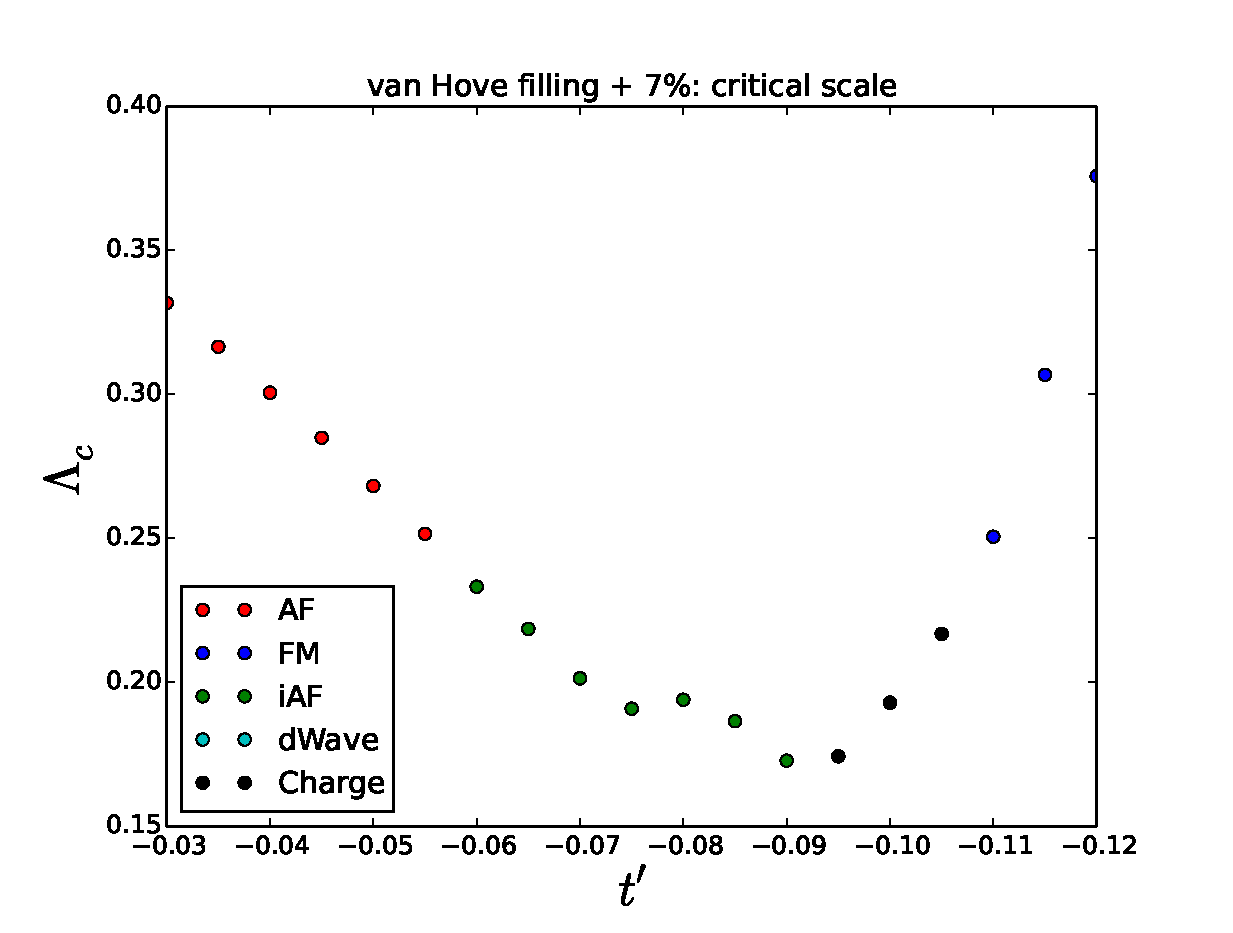
\includegraphics[scale=0.7]{vanHove_plus_scan_critical_lambda_phi.eps}
\caption{Critical scale in full frequency fRG (interaction cutoff) as a function of the nearest neighbors hopping and for van Hove filling + 7 \%. The color of the symbol indicates the kind of instability that is realized.} 
\label{phasediag_van_hove_plus} 
\end{figure}



In the spirit of the "interaction cutoff" the critical scale can be associated with the maximal value of the interaction $U_{\mathrm{flow}}\approx(1-\Lambda)^2 U$  for which the flow would converge (at the given temperature). 

In a purely weak coupling scenario one can assume a monotonic relation between the interaction value and the critical temperature, and hence we can loosely associate the critical scale whit a critical temperature.

We have double-checked the consistency of our results by also considering a frequency selective cuffoff, which substitutes: $i\omega \rightarrow i\mathrm{sign} \omega \sqrt{\omega^2+\Lambda^2}$. 

\begin{figure}
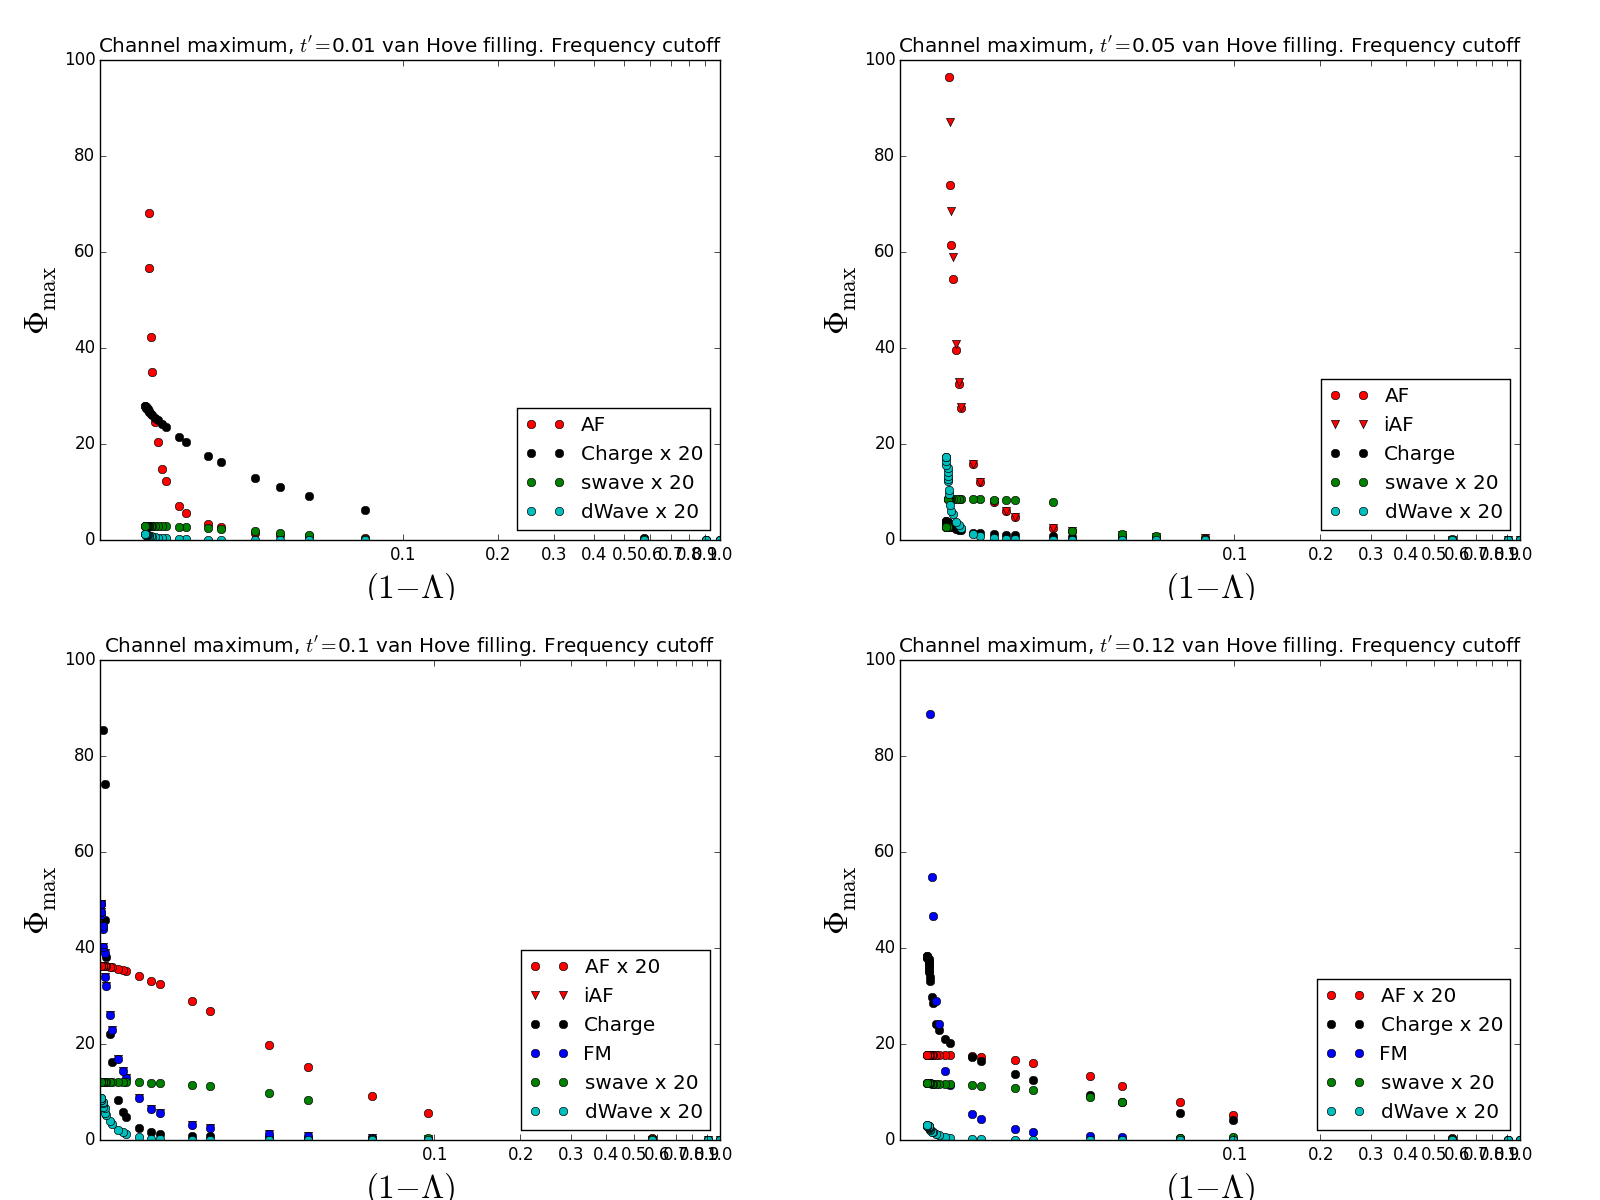
\includegraphics[scale=0.32,angle =90]{images/freqvanhove.png}
\caption{\textbf{frequency cutoff} Flow of the maximum of the absolute value of each channel for different values of $t'$ and at van Hove filling. } 
\label{freqlam} 
\end{figure}

\begin{figure}
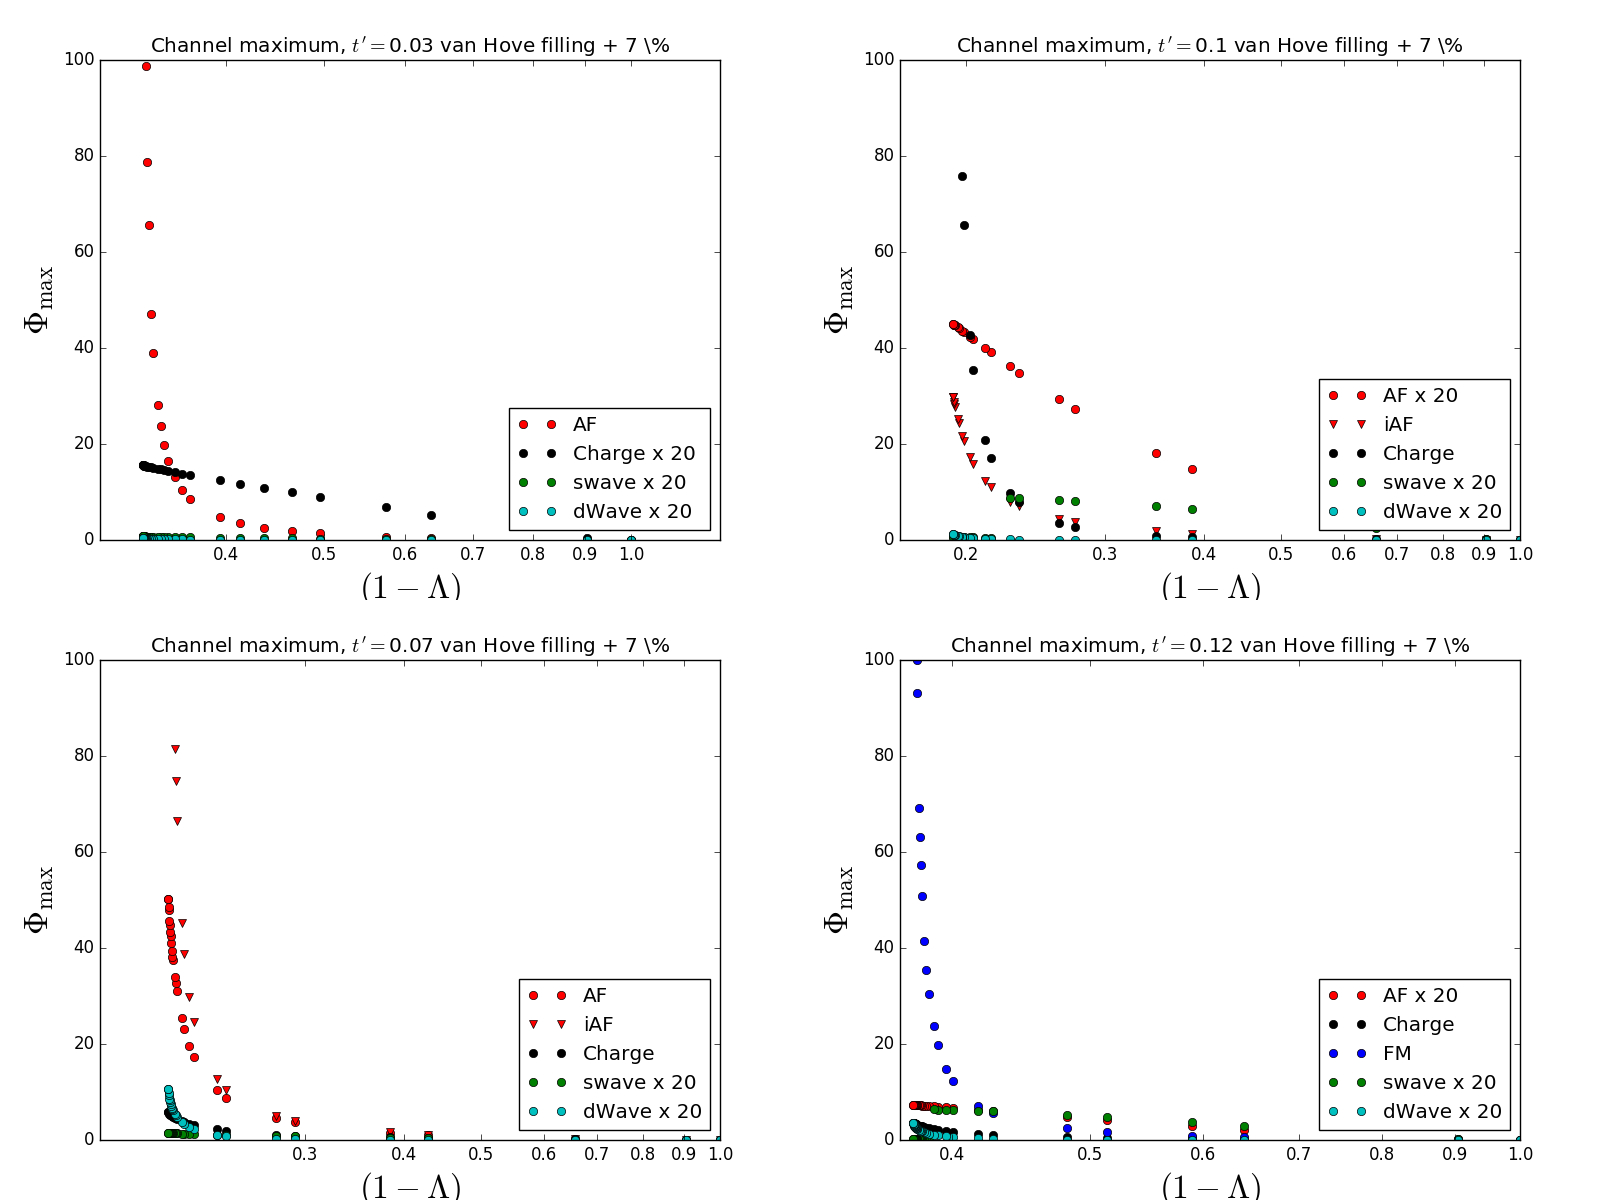
\includegraphics[scale=0.32,angle =90]{images/vanhovepluslambda.png}
\caption{Flow of the maximum of the absolute value of each channel for different values of $t'$ and at van Hove filling $+7 \%$.
} 
\label{lamvanplus} 
\end{figure}

\subparagraph{Charge instability problem}
 
\begin{itemize}
\item The charge-channel diverges for frequency transfer: $\Omega=2\pi/\beta$. 


\item The charge channel diverges for a region of filling/next neighbors hopping between iAF and FM. In static fRG in this region one can find $d$wave superconductivity, usually at much lower scales (see Figs. \ref{phasediag_van_hove}, \ref{phasediag_van_hove_plus}, \ref{phasediag_van_hoveSTATIC}).


\item The divergence of the charge channel seems to appear at the transition between iAF and FM instabilities. 

\item In Fig. \ref{phasediag_van_hove} and Fig. \ref{phasediag_van_hove_plus} it appears that the divergence points of the charge channel and of the ferromagnetism are on the same line. 

\item In Fig. \ref{lamvan} and \ref{lamvanplus} one can see that the flow of the max in the charge-channel follows the maximum in the Ferromagnetism. 

\item as a function of $t'$ it seems that the charge divergence arises as soon it appears a local maximum close to $0,0$ in the magnetic susceptibility, see Fig. \ref{susceptibilityfrg}. 
\begin{figure}
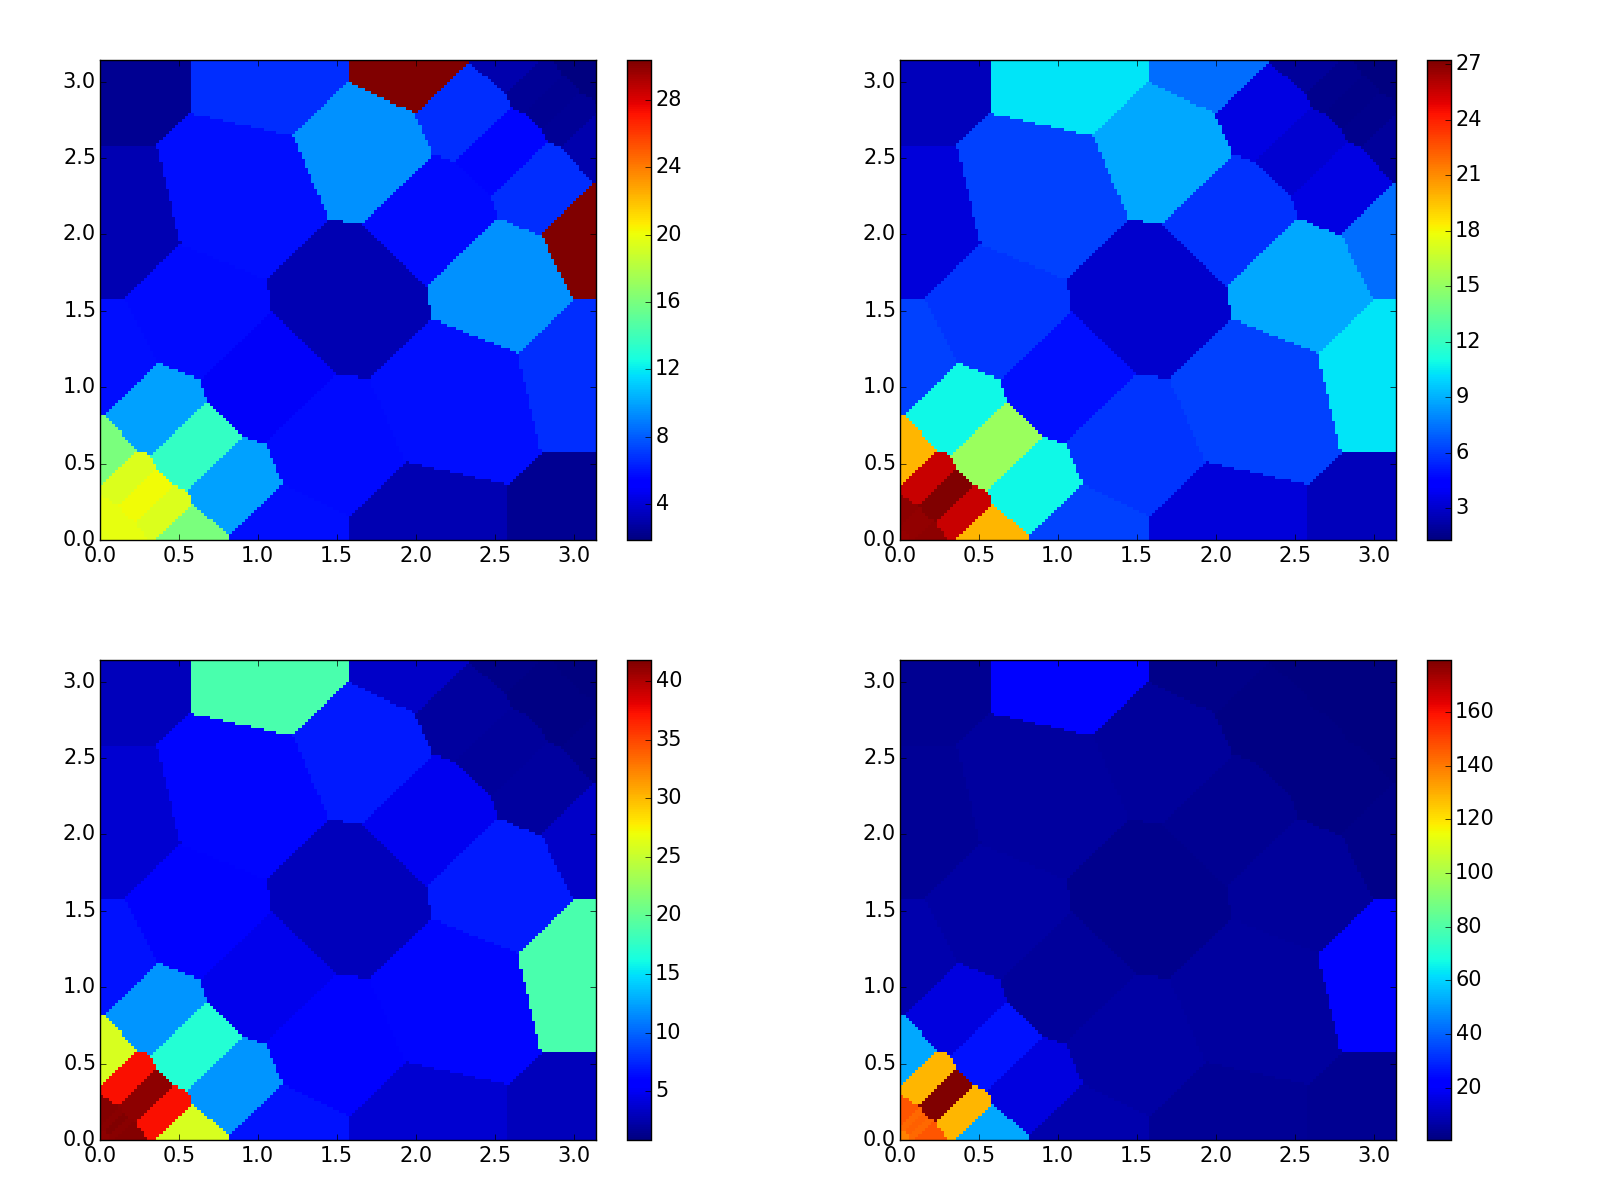
\includegraphics[scale=0.25]{images/susceptibilityfrg.png}
\caption{ Magnetic susceptibility  in the BZ computed by fRG, for the $t'$ points where the charge channel shows the divergence. 
Top $t'=-0.09t$ (left), $t'=-0.095$ (right). Bottom $t'=-0.100$ (left), $t'=-0.105$ (right). Note that the increasing the next neighbors hopping the maxima in the susceptibility shift more to the region near $\mathbf{Q} = 0,0$.
 } 
\label{susceptibilityfrg} 
\end{figure}
%\item We observed the charge channel divergence also in region away from van Hove filling, where the Ferromagnetism is suppressed (not shown). 
 
\item The \textit{divergence} of the channel is associated with a very specific \textit{frequency-structure}. The frequency-structure can be explained (section about perpendicular ladders). 
The frequency structure of the magnetic channel is rather flat, which can be interpreted in terms of RPA.
 
 \item The divergence in the charge channel is very localized in frequency space. 
Nevertheless, it is sufficient to induce large values of the charge susceptibility,  with a maximum at finite frequency transfer. This susceptibility is however never the dominant one. 
The magnetic susceptibility is larger due to the flat frequency structure of the magnetic vertex. 
 
\item The charge-channel divergence arises also in DMF$^2$RG at strong coupling, where the DMFT self-energy is already included in the flow equations.

\item Introducing a \emph{full} self-energy feedback the in DMF$^2$RG the problem seems to be suppressed. 

     
\end{itemize} 
 
\begin{figure}
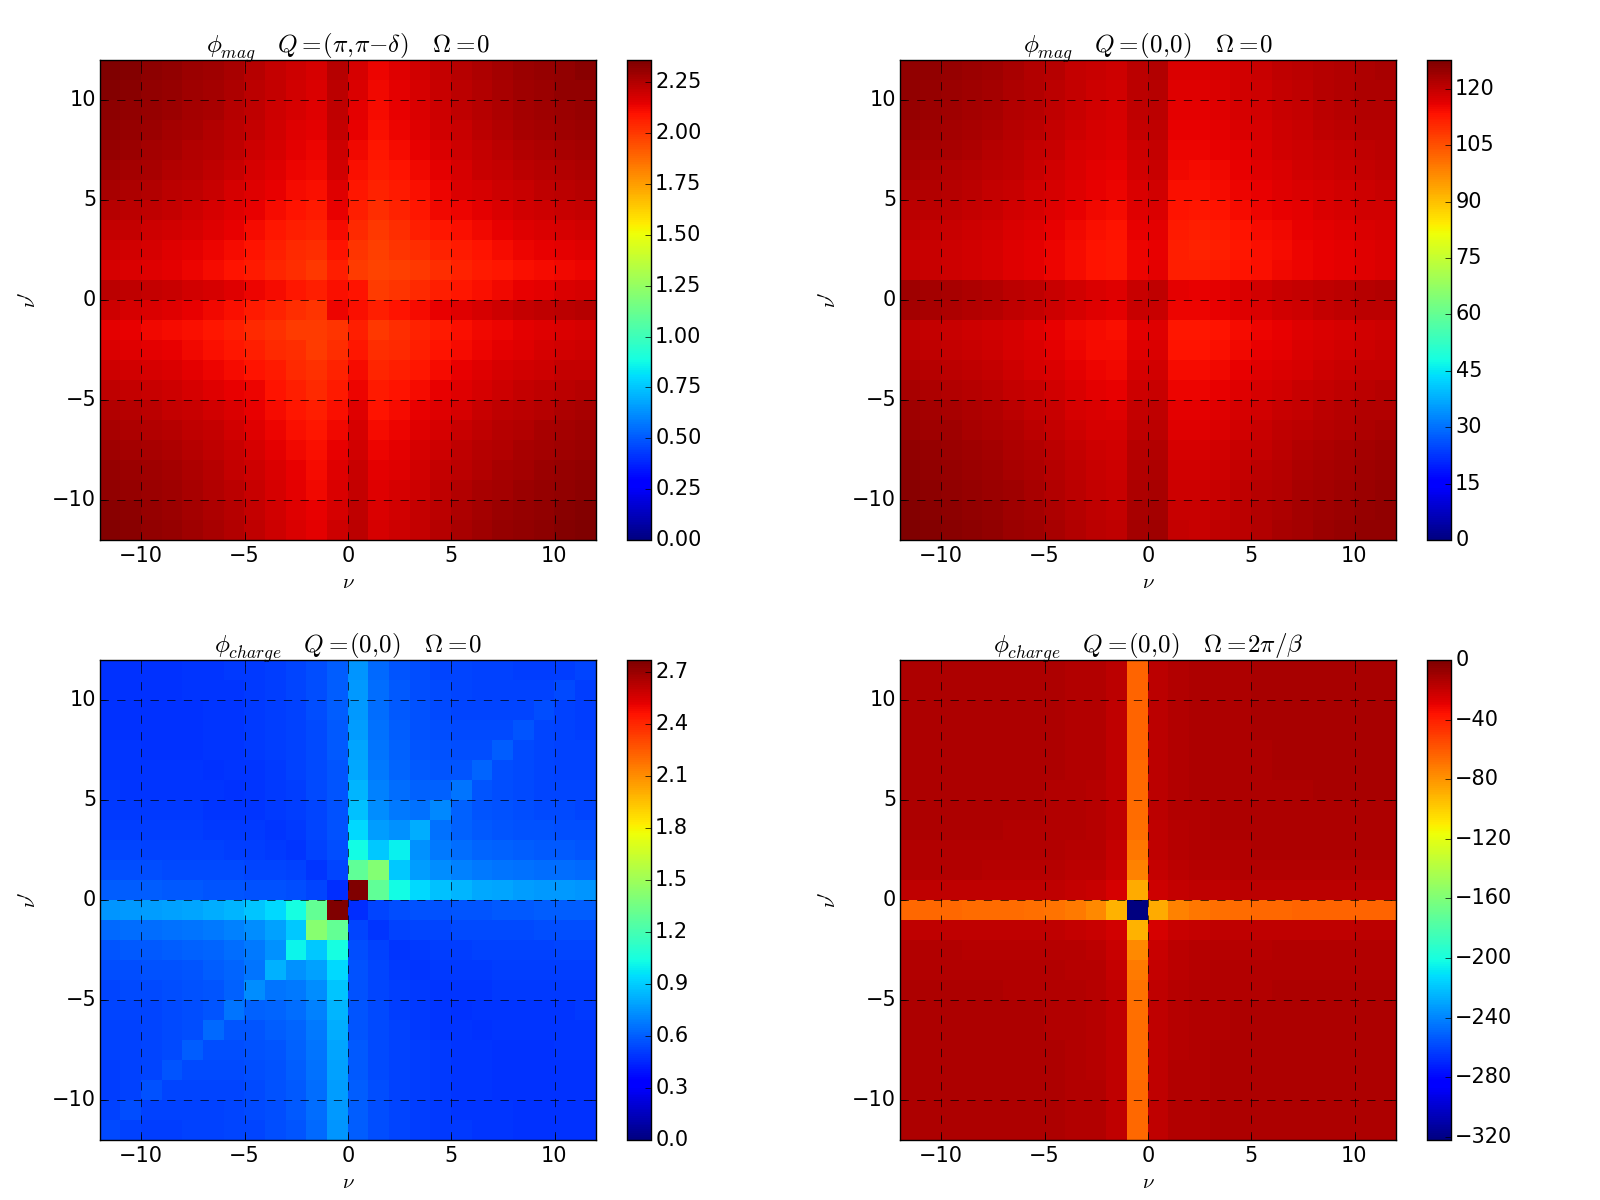
\includegraphics[scale=0.3]{images/Merged_tpri0105.png}
\caption{Frequency structure of the channels. Top left: magnetic channel for momentum closet to $\pi,\pi$ where the vertex has a local maximum, top right: magnetic channel for momentum close to $0,0$, in both cases external frequency transfer $\Omega=0$. 
Bottom left: charge channel for external frequency transfer $\Omega=0$ and transfer momentum $0,0$, bottom right: the same but for \emph{finite} frequency transfer $\Omega = 2\pi/\beta$. } 
\label{structurechargefrg} 
\end{figure}
